\chapter{Tracing the execution}

\section*{Introduction}

The code of Trampoline RTOS embeds a tracing subsystem that can be activated at
system configuration time.
This toolkit sends a stream of events describing the execution of the
application to a target specific backend.
The resulting data can then be exploited to compute statistics on some
performance figures of the system (such as execution times, jitters, etc.)
and/or to feed a visualization tool.
Please notice that, in the current implementation, the tracing toolkit has a small, albeit non null, overhead so
the system from which traces are computed is not exactly the same than the
system without traces.

\section{Traced events}


Events that can be traced during an execution are given below.
Each event is described by its name and a set of attributes.
These attributes are made available by the kernel to the platform specific
backend (see section~\ref{sec:trace:targetbackend} below).

\begin{description}
  \item[TRACE\_PROC]: state of a process (task or ISR) is changed.
    \begin{itemize}
      \item \texttt{proc\_id}: identifier of the process.
      \item \texttt{target\_state}: new state of the proc. %TODO: list states
    \end{itemize}

  \item[TRACE\_RES]: state of a resource is changed.
    \begin{itemize}
      \item \texttt{res\_id}: identifier of the resource.
      \item \texttt{target\_state}: new state of the resource. %TODO: list states
    \end{itemize}

  \item[TRACE\_EVENT]: a process set/reset one or more event to another process.
    \begin{itemize}
	  \item \texttt{proc\_id}: owner of the events (when event is set)
      \item \texttt{ev\_id}: list of events that have been set.
    \end{itemize}

  \item[TRACE\_ALARM]: state of a timeobj (alarm, schedule table
    expiry point) is changed.
    \begin{itemize}
      \item \texttt{timeobj\_id}: identifier of the timeobj.
	  \item \texttt{kind}: change state or expire.
    \end{itemize}

  \item[TRACE\_MESSAGE]: a message is sent or received.
    \begin{itemize}
      \item \texttt{msg\_id}: identifier of the message
	  \item \texttt{kind}: kind of message (receive, send, send 0 message)
    \end{itemize}
  \item[TRACE\_IOC]: **not well tested**
  \begin{itemize}
  	\item \texttt{mess\_id}: identifier of the message.
  \end{itemize}
  

\end{description}

Notice that each event contains the minimal information that is needed
to rebuild the whole state of the system.
Hence, the running task is never used as an attribute because it can be deduced
by analysing the sequence of \emph{TRACE\_PROC} events.

\section{OIL declaration}
\subsection{Generic part}

Activation of tracing is done at system configuration time through the OIL file.
A boolean attribute \texttt{TRACE} is defined in the \texttt{OS} object. It has
several subattributes has shown in the code below:

\begin{lstlisting}[language=OIL]
TRACE = TRUE {
    FORMAT = SERIAL;
    PROC = TRUE;
    RESOURCE = TRUE;
    ALARM = TRUE;
    EVENT = TRUE;
    MESSAGE = TRUE;
};
\end{lstlisting}

\begin{description}
	\item[FORMAT] specifies the output format of the trace. This is a target dependant attribute. For instance, the posix target allows the \texttt{json} output, while the msp430 allows the \texttt{serial} and \texttt{fram} targets (with sub-attributes). See section \ref{sec:traceTargetFormat}.

\end{description}
The other sub-attributes define types of events to trace: \texttt{PROC}, \texttt{RESOURCE}, \texttt{ALARM}, \texttt{EVENT}, \texttt{MESSAGE}, \texttt{IOC}

\subsection{Target specific part}
\label{sec:traceTargetFormat}
\subsubsection{Posix target}
The posix target is the simplest one, as there is no problem to get back the trace. The trace can be saved in \texttt{json} mode only. The generated file is always called \texttt{trace.json}.


\subsubsection{MSP430 target}
For the MSP430 format, different methods can be implemented to retrieve the trace:
\begin{description}
	\item[\texttt{SERIAL}] the serial communication, using the \emph{serial over USB} link on launchpad dev board;
	\item[\texttt{FRAM}] the FRAM storage. In that case, the trace is stored directly on the FRAM and can be read using a gdb dump. Sub-attributs are:
\begin{description}
	\item[\texttt{SIZE}] the size of the dump in bytes;
	\item[\texttt{ADDRESS}] the base address.
\end{description} It should not be used if the throughput is too high!
(\emph{not implemented yet}).

	\item[\texttt{SD}] the embedded SD card (\emph{not implemented yet}).
\end{description}

In all cases, a trace event should take as low place as possible, and is stored in binary format (see section \ref{sec:traceBinFormat}).

\subsubsection{STM32 target}
On STM32 (Nucleo STM32F303 and STM32L432), the Serial target is implemented. There is a full example in \texttt{examples/cortex/armv7em/stm32f303/Nucleo-32/trace}

\begin{lstlisting}[language=OIL]
    TRACE = TRUE {
        FORMAT   = serial;
        PROC     = TRUE;
        RESOURCE = TRUE;
        ALARM    = TRUE;
        EVENT    = TRUE;
    };
    
    BUILD = TRUE {
	  //..
      LIBRARY = serial {TXBUFFER = 256;};
	  //..

\end{lstlisting}

\subsubsection{Arduino Uno target}
On Arduino UNO, the Serial target is implemented (using the arduino Serial driver).
There is a full example in \texttt{examples/avr/arduinoUno/trace}

\section{Using the tracing subsystem}

The trace are generated by trampoline on the target. We then need to retrieve the information on the host system. 

The trace system is split in 3 steps, as defined in Figure \ref{fig:trace}:
\begin{description}
	\item[TraceReader] reads \textsl{raw events} from the target. A \textsl{raw event} deals only with numerical ids from Trampoline. The reader can read events from the serial or from a file at this date. It can store them to a file for later evaluation.
	\item[TraceEvaluate] associates a name with each ids, thanks to the \lstinline{tpl_static_info.json} file generated by goil. It can make some extra evaluation on the application: there is never an event received by a suspended task, there is no critical section overlap due to bad resource usage, a task that gets a resource has the right to do so, …
	\item[TraceAnalysis] analysis of the trace: cpu load, event listing, …
\end{description}

\begin{figure}[htbp]
    \centering
	\begin{adjustbox}{width=.7\linewidth,keepaspectratio}
		\definecolor{WPAColor}{RGB}{218,232,252}     %DAE8FC => 218 232 252
\definecolor{WPAColorLine}{RGB}{108,142,191} %6C8EBF => 108 142 191
\definecolor{WPBColor}{RGB}{213,232,212}     %D5E8D4 => 213 232 212
\definecolor{WPBColorLine}{RGB}{130,179,102} %82B366 => 130 179 102
\definecolor{WPCColor}{RGB}{230,230,230}     %E6E6E6 => 230 230 230
\definecolor{WPCColorLine}{RGB}{182,182,182} %B6B6B6 => 182 182 182
\definecolor{WPDColor}{RGB}{255,233,212}     %FFE9D4 => 255 233 212
\definecolor{WPDColorLine}{RGB}{148,135,123} %94877B => 148 135 123

\begin{tikzpicture}[
WPA/.style ={WPAColorLine,fill=WPAColor,thick}, 
WPB/.style ={WPBColorLine,fill=WPBColor,thick},
WPC/.style ={WPCColorLine,fill=WPCColor,thick},
WPD/.style ={WPDColorLine,fill=WPDColor,thick},
txt/.style = {font=\Large},
boxTxt/.style = {txt,text width=3cm, text centered,text=black},
box/.style ={draw,drop shadow={opacity=0.25},boxTxt,minimum height=2cm,minimum width=3.8cm},
cercle/.style ={draw,circle,drop shadow={opacity=0.25},boxTxt,minimum height=3cm,minimum width=3.5cm},
boxLegende/.style={box,minimum width=1.5cm,text width = 0cm,minimum height=1cm},
fleche/.style={->,>=stealth,line width=0.5mm},
srcFile/.style={draw,tape,drop shadow={opacity=0.25},boxTxt, minimum height=1.3cm, tape bend top=out and in, tape bend bottom=out and in}
]

  \node[WPB,srcFile,text width = 3cm] (traceJson) at (-5,3) {\texttt{trace.json}};
  \node[WPA,srcFile,text width = 6cm] (traceStaticJson) at (-7,1) {\texttt{tpl\_static\_info.json}};
  \node[WPD,srcFile,text width = 3cm] (traceTarget) at (0,7) {compressed event list};
  \node[fill=WPCColor,box,minimum height=1cm] (TraceReader)   at (0,3) {\texttt{TraceReader}};
  \node[fill=WPCColor,box,minimum height=1cm] (TraceEvaluate) at (0,0) {\texttt{TraceEvaluate}};
  \node[fill=WPCColor,box,minimum height=1cm] (TraceExport)   at (0,-3) {\texttt{TraceExport}};

  \draw[fleche] (traceJson) to[bend left] (TraceReader);
  \draw[fleche] (TraceReader) to[bend left] (traceJson);
  \draw[fleche] (TraceReader) -- (TraceEvaluate) node[midway,right] {event list with ids}; ;


  \draw[fleche] (traceStaticJson) -- (TraceEvaluate) node[midway,below left] {id $\Leftrightarrow$ name}; 
  \draw[fleche] (TraceEvaluate) -- (TraceExport) node[midway,right] {event list with names}; 
 % \draw[fleche] (readBin) -- (traceJson) node[midway,right] {event list}; 

  \draw[fleche,<-] ($(TraceReader.north)+( 1,0)$) -- ($(traceTarget.south)+(+1,0)$) node[midway,right,text width = 2cm] {serial comm}; 
  \draw[fleche,<-] ($(TraceReader.north)+(-.4,0)$) -- ($(traceTarget.south)+(-.4,0)$) node[midway,left ,text width = 2cm] {gdb binary dump}; 
  \draw[fleche,<-] ($(TraceReader.north)+(0.3,0)$) -- ($(traceTarget.south)+(0.3,0)$) node[midway,left] {…}; 
  \draw[line width=0.2mm,dashed] (-10,6.5) -- ++(0,-1) node[above right] {target}-- ++(13,0) -- ++(0,1);
  \draw[line width=0.2mm,dashed] (-10,3.3) -- ++(0,+1) node[below right] {host}-- ++(13,0) -- ++(0,-1);
  \draw[fleche] (TraceExport) -- ++(0,-1) node[below] {event list (text based, gui)};

\end{tikzpicture}

	\end{adjustbox}
	\caption{Getting trace list from the target. The \lstinline{readTrace.py} script calls the 3 steps of the trace : \lstinline{TraceReader}, \lstinline{TraceEvaluate} and \lstinline{TraceAnalysis}, for each event.}
	\label{fig:trace}
\end{figure}

For the serial line reader, the events are queued in a dedicated thread, so that there is no event loss, even if evaluation/analysis are too slow.

\note{On the posix target, trampoline generates directly the \texttt{trace.json} file.}

Tools are provided in the \texttt{extra/trace-tools/} directory of Trampoline, and called directly by the generated script \lstinline{readTrace.py}. Run to have information how to use the script:

\begin{lstlisting}
./readTrace.py --help
\end{lstlisting}

For now, the script can read from a json file (posix or saved trace) or a serial line. It can save a received trace to a file for later use (raw events). The analysis for now just gives the list of events or calculate the cpu load.

\note{When receiving an endless trace (serial line for instance), you can terminate the reception with \texttt{Ctrl+C}}.

\section{Implementation}
The implementation is split in 2 parts:
\begin{itemize}
	\item the \emph{generic} part is a set of macro in the \texttt{os/} kernel files to captures trace events. The file \texttt{os/tpl_trace.h} list all the specific functions that should be implemented.
	\item the \emph{target specific} part in \lstinline{machine/.../tpl_trace.c} implements the trace back-end. 
\end{itemize}

\subsection{Implementing target specific backends}
\label{sec:trace:targetbackend}

The backend consists in a set of 7 functions that should be implemented in the target to store events, and communicate them to an host computer for analysis. Prototypes are in the \texttt{os/tpl_trace.h} are each function is related to a trace event. For instance, the following function will be called by the kernel internal files (\emph{in kernel mode!}) each time a proc (task/isr) state is updated.

\begin{lstlisting}
/**
* trace the execution of a task or ISR
* This function should be implemented in the machine dependant trace backend.
*
*/
FUNC(void, OS_CODE) tpl_trace_proc_change_state(
    CONST(tpl_proc_id,AUTOMATIC) proc_id,
    CONST(tpl_proc_state,AUTOMATIC) target_state);
\end{lstlisting}

A new file is now generated by goil \texttt{tpl_static_info.oil} that lists the objects defined in the oil file. This file can be combined with the trace to deal with the name of an object instead of its internal id.


\subsection{Binary format}
\label{sec:traceBinFormat}

The binary format is defined in Figure \ref{fig:traceBin}. It is composed of:
\begin{description}
	\item[Type]\footnote{defined in \lstinline{os/tpl_trace.h}} There are 7 events types: 
		\begin{itemize}
			\item PROC\_TYPE: a task/isr2 changes its state (running, suspended, ready,…);
			\item RES\_TYPE: related to resources (\lstinline{getResource}/\lstinline{ReleaseResource})
			\item EVENT\_TYPE: related to events (\lstinline{SetEvent}/\lstinline{ReleaseEvent})
			\item TIMEOBJ\_TYPE: related to alarms and schedule tables (\lstinline{SetRelAlarm}, \lstinline{CancelAlarm}, …)
			\item MESSAGE\_TYPE: related to communication (\lstinline{GetMessage}/\lstinline{ReceiveMessage})
			\item IOC\_TYPE: related to IOC (AutoSar extension) 
		\end{itemize}
		One extra type \emph{OVERFLOW\_TYPE} is defined if the communication medium cannot provide a sufficient bandwidth. 3 bits are required.
	\item[TimeStamp] The time stamp. The overflow should be taken into account by the receiver (events are in chronological order). Most significant byte first.
	\item[xxx] This is the event dependent data (5+8 bits).
	\item[Chksum] The checksum (8 bits) is the sum of the 4 previous bytes. Its goal is both to detect errors and frame limits.
\end{description}

\begin{figure}[htbp]
    \centering
	\begin{adjustbox}{width=.8\linewidth,keepaspectratio}
		\definecolor{colorLine}{RGB}{100,100,100}
\definecolor{colorFill}{RGB}{230,230,230}

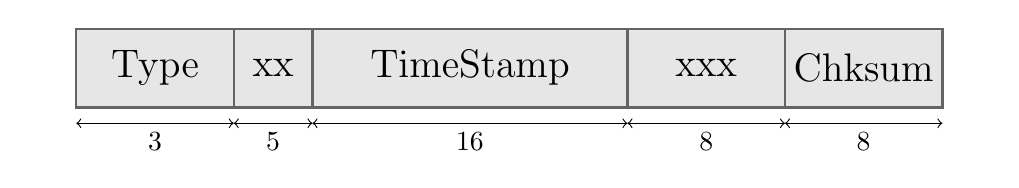
\begin{tikzpicture}[
txt/.style = {font=\Large},
boxTxt/.style = {colorLine,fill=colorFill,thick,txt,text width=3cm, text centered,text=black},
box/.style ={draw,drop shadow={opacity=0.25},boxTxt,minimum height=2cm,minimum width=3cm},
boxLegende/.style={box,minimum width=1.5cm,text width = 0cm,minimum height=1cm},
fleche/.style={->,>=stealth,line width=0.5mm},
srcFile/.style={draw,tape,drop shadow={opacity=0.25},boxTxt, minimum height=2cm, tape bend top=out and in, tape bend bottom=out and in}
]

%w    width is displayed frame
%text field text
%s    size in trace
\newcount\offset
\offset=0
\foreach \w/\text/\s in {
  2/Type      /3,
  1/xx        /5,
  4/TimeStamp/16,
  2/xxx       /8,
  2/Chksum    /8
}{
  \draw[boxTxt] (\the\offset,0) rectangle ++(\w,1) node[midway] {\text};
  \draw[<->] (\the\offset,-.2) -- ++(\w,0) node[midway,below] {\s};
  \global\advance\offset by \w
}

\end{tikzpicture}

	\end{adjustbox}
	\caption{binary format of a trace event (5 bytes)}
	\label{fig:traceBin}
\end{figure}

For each type, we define the specific bits:

\begin{table}[htbp]
	\rowcolors{1}{white}{light-gray}
	\begin{longtable}[c]{c|c|l}
		\bf Type & \bf format (5+8 bits) & \bf fields \\ \hline
		PROC\_TYPE    & \texttt{00SSS PPPPPPPP} & \texttt{S} (3 bits): proc state      \\
		              &                         & \texttt{P} (8 bits): proc id         \\ \hline
		RES\_TYPE     & \texttt{0000S RRRRRRRR} & \texttt{S} (1 bit ): res state (free/taken)       \\
		              &                         & \texttt{R} (8 bits): res id          \\ \hline
		EVENT\_TYPE   & \texttt{EEEEE KTTTTTTT} & \texttt{E} (5 bits): event id        \\
		              &                         & \texttt{K} (1 bit) : kind            \\ 
		              &                         & \texttt{T} (8 bits): task id         \\ \hline
		TIMEOBJ\_TYPE & \texttt{K0SSS TTTTTTTT} & \texttt{K} (1 bit) : kind            \\
		              &                         & \texttt{S} (3 bits): time obj. state \\
		              &                         & \texttt{T} (7 bits): time obj id     \\ \hline
		MESSAGE\_TYPE & \texttt{MMMMM 000000KK} & \texttt{M} (5 bits): message id      \\
	                  &                         & \texttt{K} (2 bits): kind            \\ \hline
		%IOC\_TYPE     & \texttt{MMMMM 000000TT} & \texttt{M} (5 bits): message id \\
	\end{longtable}
	\caption{Specific bits for each event type}
	\label{tab:traceBin}
\end{table}


Due to frame size limits, the number of events is limited to 31, the number of procs (task/isr) to 255, as well as time objects (alarms, schedule tables) and resources.

Some types have a sub-type (kind):
\begin{description}
	\item[EVENT\_TYPE] kind may be \texttt{0} when an event is set or \texttt{1} when the event is reset (there is no \texttt{task id} as it is the running task. 
	%\item[TIMEOBJ\_TYPE] kind may be \texttt{0} when an event is set or \texttt{1} when the event is reset (there is no \texttt{task id} as it is the running task. 
	%\item[MESSAGE\_TYPE] kind may be \texttt{0} when an event is set or \texttt{1} when the event is reset (there is no \texttt{task id} as it is the running task. 
\end{description}


The message event type bits is used to indicate the specific type of event associated with the message, such as send and receive.

\subsection{How to port \texttt{trace} to another target}

The \texttt{tpl\_trace.c} is target specific. It should be defined in the \lstinline{machine} hierarchy. A good starting point is the stm32's version\footnote{file \texttt{machines/cortex/armv7em/stm32f303/tpl_trace.c}}, with a SERIAL implementation. In the \texttt{avr/arduino} version, a C++ example is provided.

Then, the goil templates should be updated. This is done in 2 steps:

\begin{itemize}
	\item Add the new file \texttt{tpl\_trace.c} (or \texttt{.cpp}) to be compiled in the project: in \texttt{config/\textit{target}/config.oil} \\
\begin{lstlisting}
  PLATFORM_FILES targetTrace {
    PATH    = "target";        //path, starting from machine/
    CFILE   = "tpl_trace.c";   // file name (cpp allowed)
  };
\end{lstlisting}

	\item Add the definition of the trace type to be defined in the oil file: in section IMPLEMENTATION/OS in \texttt{config/\textit{target}/config.oil}:
\begin{lstlisting}
    /* trace */
    BOOLEAN [
      TRUE {
        ENUM [
          serial
        ] FORMAT = serial;
      },
      FALSE
    ] TRACE = FALSE;
\end{lstlisting}
\end{itemize}

In this example, only the serial type is allowed. You can have a look to the msp430 version, where other modes are available, and one have sub-attributes (for fram target).

That's all!
%\subsubsection{MSP430}
%%% Local Variables:
%%% mode: latex
%%% TeX-master: "main"
%%% End:
